\documentclass[%
 reprint,
 amsmath,amssymb,
 aps,
 pra,
]{revtex4-1}

\usepackage{graphicx}% Include figure files
\usepackage{dcolumn}% Align table columns on decimal point
%\usepackage{bm}% bold math
\usepackage{fullpage}
\usepackage{epsfig}
\usepackage{amsmath}
\usepackage{amsthm}
\usepackage{amsfonts}
\usepackage{amssymb}
\usepackage{float}
\usepackage{pstricks}
\usepackage{cancel}
\usepackage{lipsum}
%\usepackage[nottoc,numbib]{tocbibind} %Uncomment for bibliography to be its own numbered section
\usepackage{units}
\usepackage{listings}
\usepackage{xfrac}
\usepackage{subcaption}

\graphicspath{{./plots/}}

\begin{document}

\preprint{APS/123-QED}

\title{\textbf{Lab Report: Phase Transitions} \\ \small{An Investigation of The VO$_2$ Metal-Insulator and BaTiO$_3$ Ferroelectric Transitions}}
\author{Joshua LaBounty}
\author{Thomas Krahulik}
\affiliation{Stony Brook University --- PHY 445}

\date{\today}

\begin{abstract}
	\lipsum[1]
\end{abstract}
\maketitle

\section{Introduction}



\section{Review of Previous Work}

\section{Experimental Setup}

\subsection{Calibration and Measurement of Internal Resistance of Lock-In Amplifier}

\subsection{Preparation of Samples}

In the course of this lab, we will make use of two different sample materials: Vanadium Dioxide (VO$_2$) and Barium Titanate (BaTiO$_3$). The Vanadium samples consist of a thin layer of VO$_2$ ($\sim 100~nm$) deposited on a silicon substrate. These Vanadium samples are pre-mounted on their electrical contacts, but we have prepared a Barium sample for our own use. Our goal with the Barium sample is to construct a parallel plate capacitor using silver paint on either side of a flat sample. In order to maximize the capacitance, in accordance with the known relation $C = \epsilon A/d$ where $\epsilon = k \epsilon_0$, we want to maximize the surface area of our sample and minimize its thickness. To that end, we chose the largest piece of Barium Titanate available and carved it down. We began by scraping thick layers of material off with a x-acto knife, and when the sample became sufficiently thin we switched to sandpaper to smooth the surface.

\begin{figure}[H]
	\centering
	\begin{subfigure}{0.22\textwidth}
		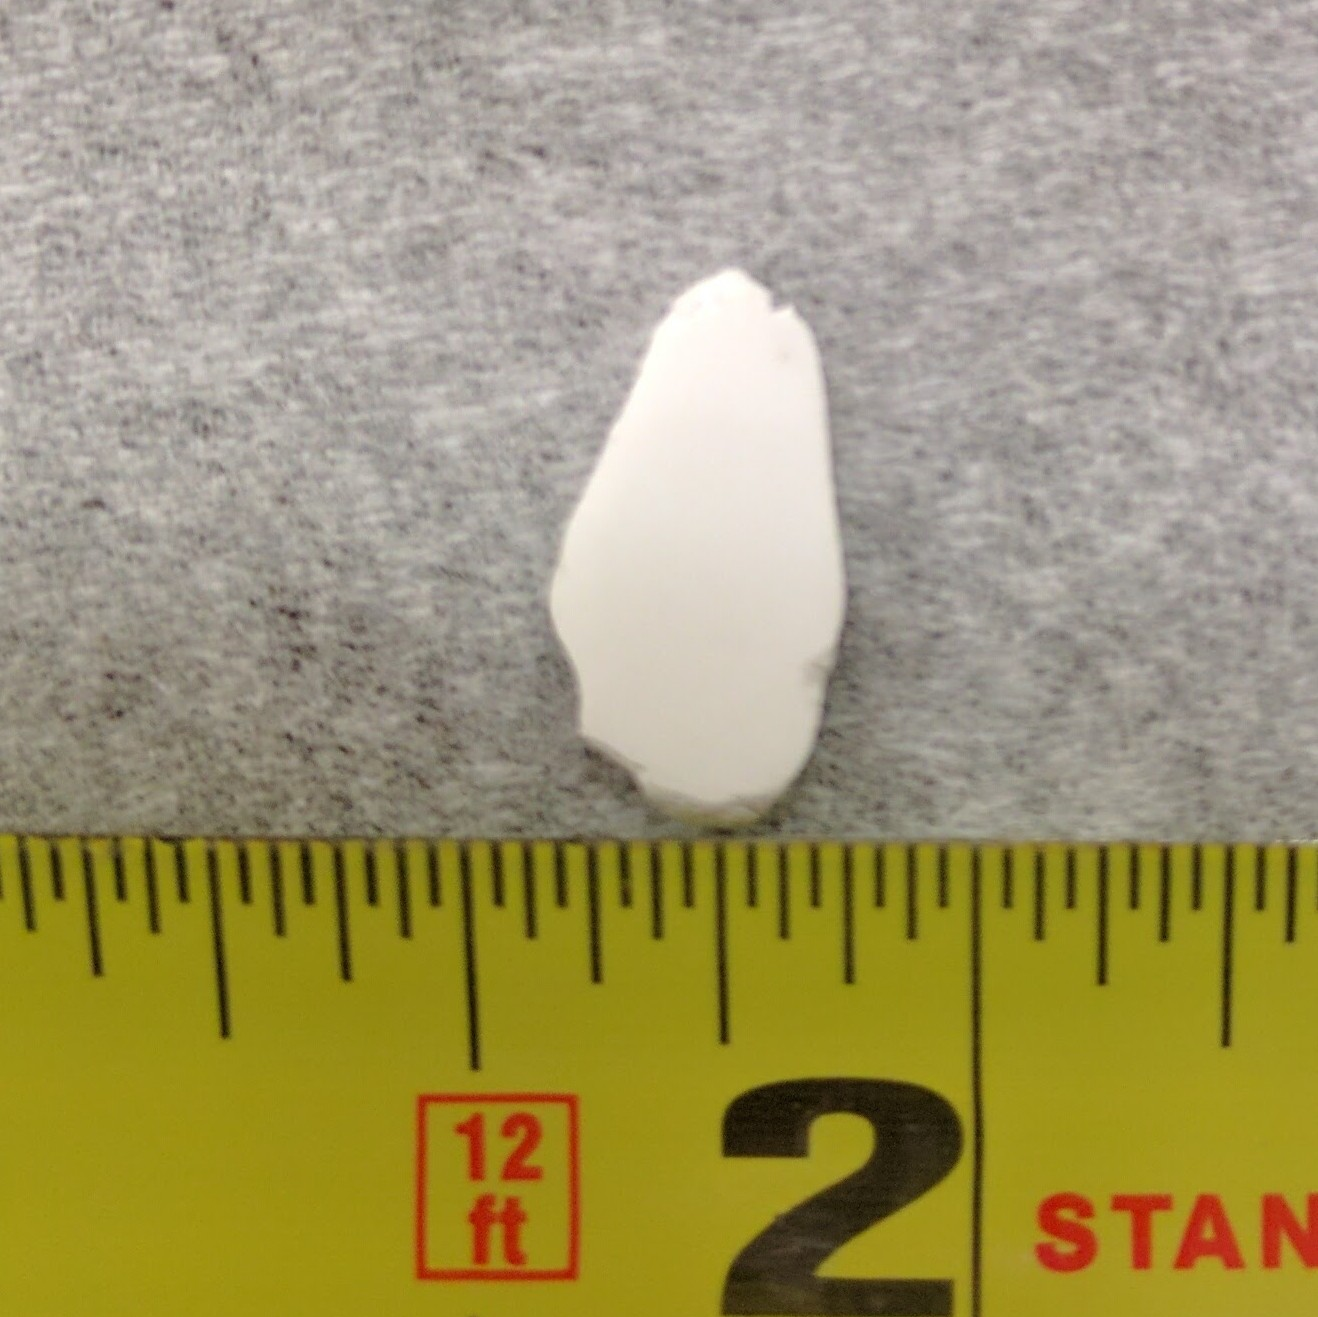
\includegraphics[width=1\textwidth]{sample_area.jpg}
		\caption{}
		\label{fig:sample:area}
	\end{subfigure}
	\begin{subfigure}{0.22\textwidth}
		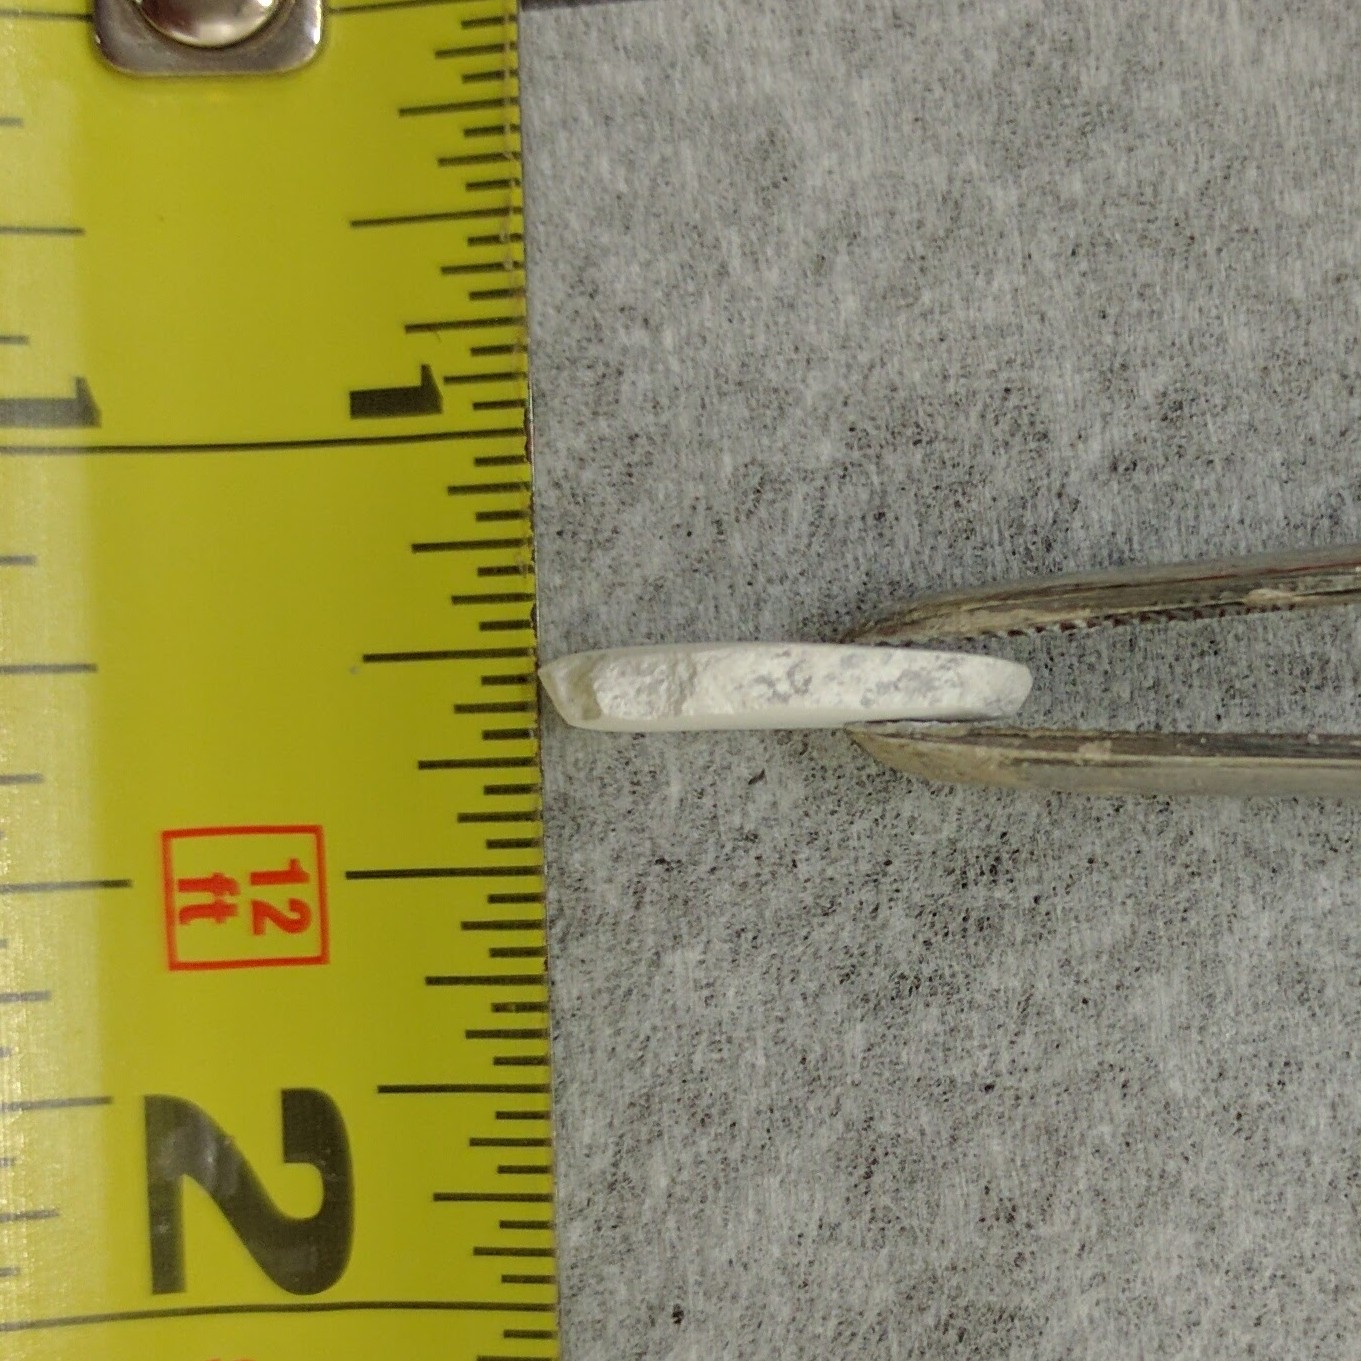
\includegraphics[width=\textwidth,angle=90]{sample_thickness.jpg} 
		\caption{}
		\label{fig:sample:thickness}
	\end{subfigure}
	\begin{subfigure}{0.22\textwidth}
		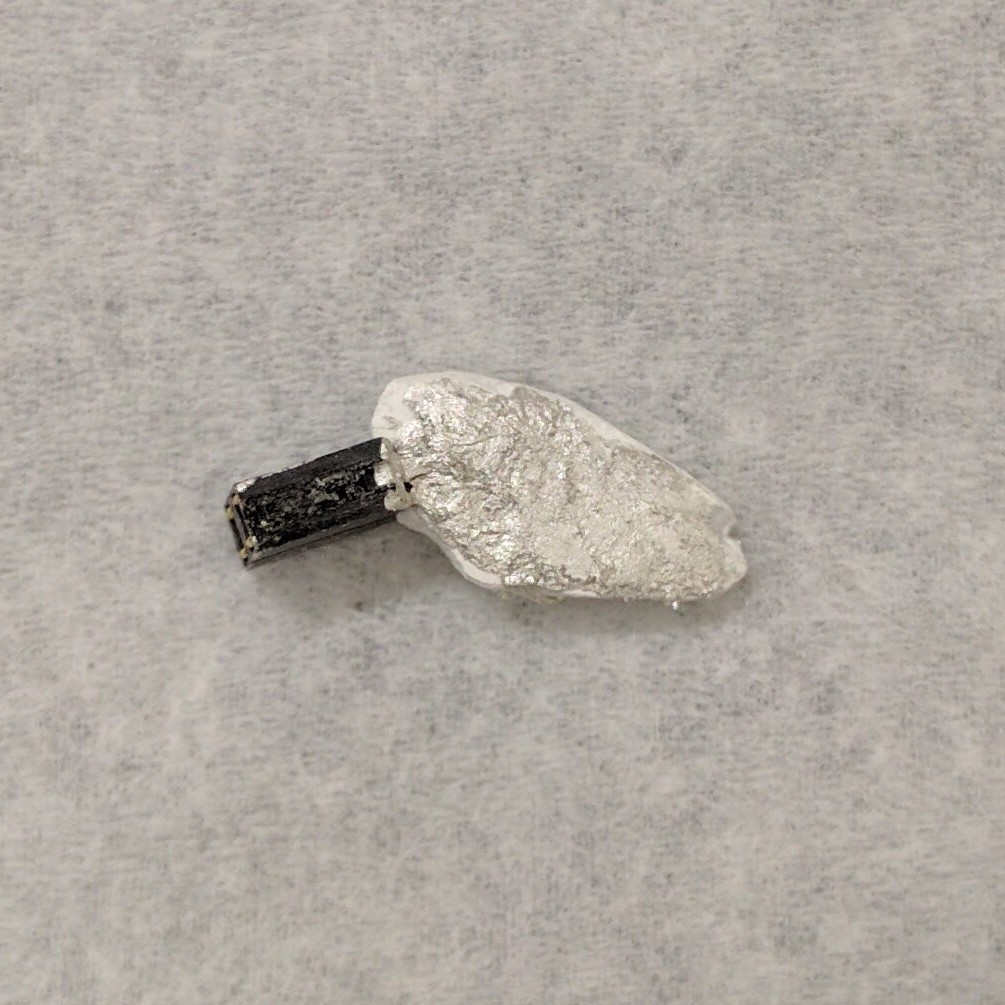
\includegraphics[width=\textwidth]{sample_complete.jpg}
		\caption{}
		\label{fig:sample:final}
	\end{subfigure}
	\begin{subfigure}{0.22\textwidth}
		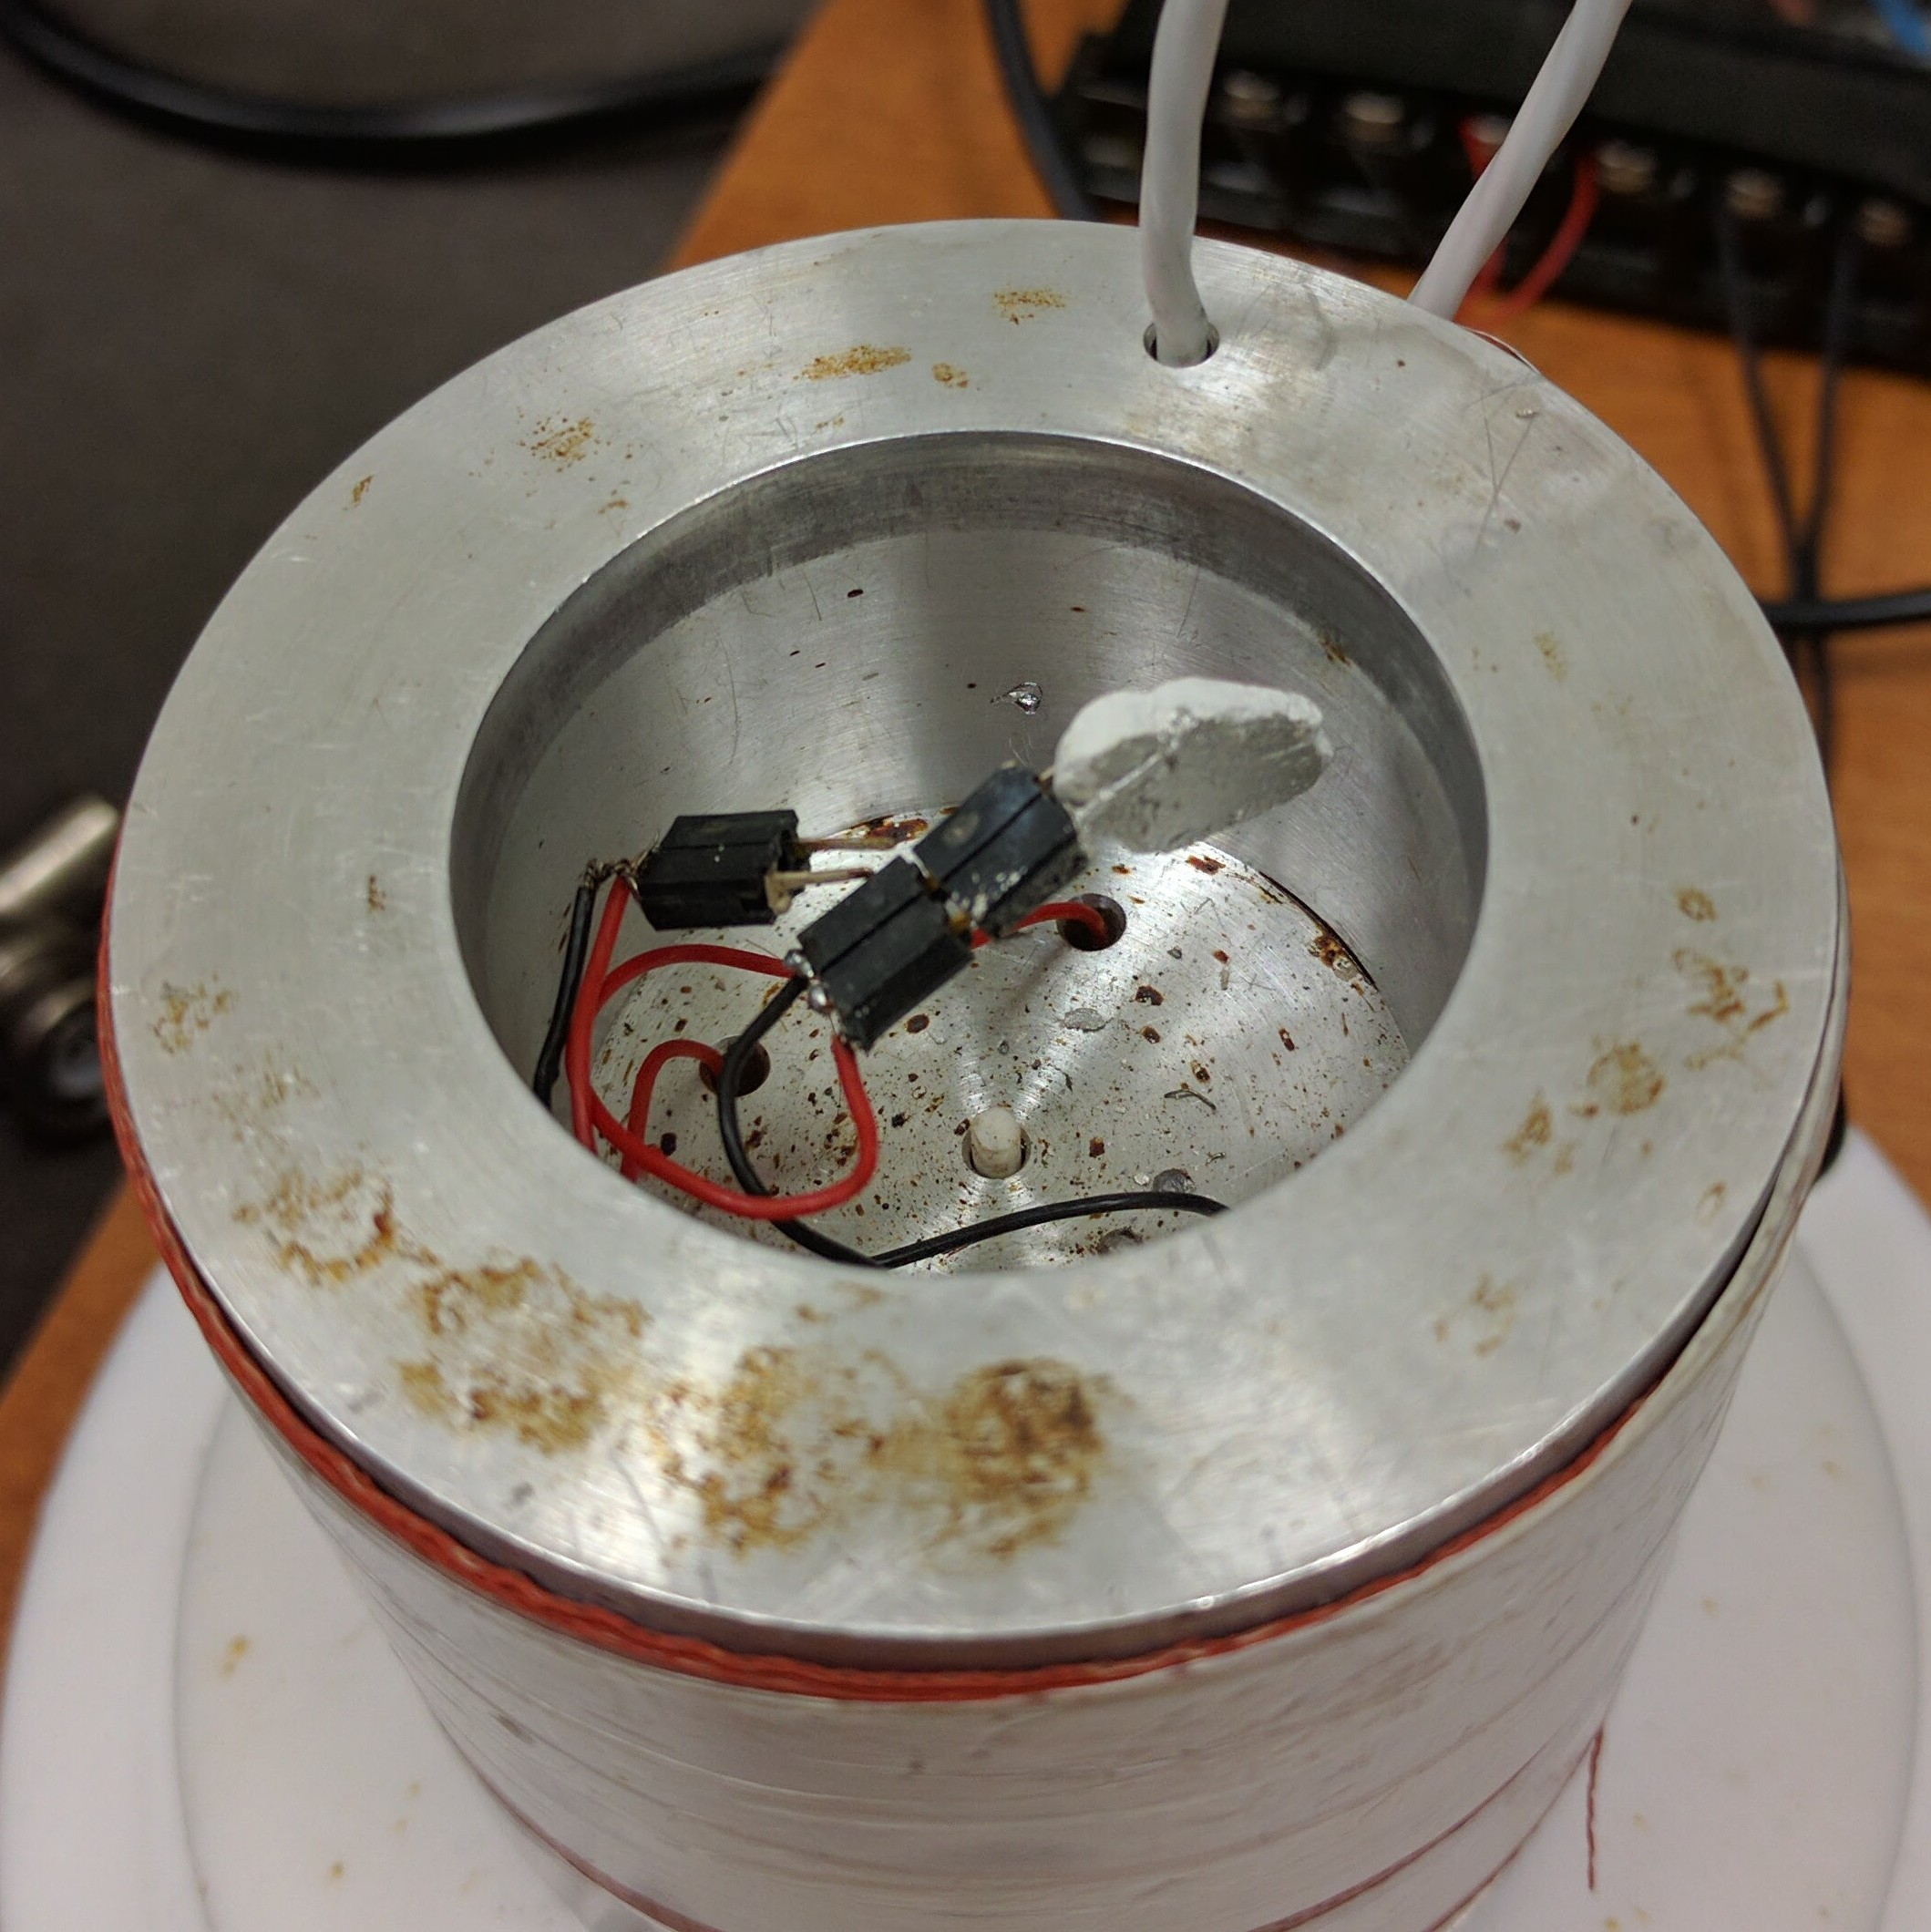
\includegraphics[width=\textwidth]{sample_inplace.jpg}
		\caption{}
		\label{fig:sample:inplace}
	\end{subfigure}
	\caption{Preparation of the Barium Titanate sample. Subfigures \ref{fig:sample:area} and \ref{fig:sample:thickness} show the images used to measure the thickness and the area of the sample. Subfigures \ref{fig:sample:final} and \ref{fig:sample:inplace} show the final sample, with the electrical connections attached by silver paint.}
	\label{fig:sample}
\end{figure}

Because we chose to maximize the area rather than creating a uniform geometric shape, whose area would have been simple to measure, we performed an indirect measurement of the area. Using a cell phone camera, we took an image with the sample and a ruler at the same distance. We used the photo editing tool GIMP to determine the surface area and thickness of the sample in pixels ($px$). We also measured the length of a section of the ruler to determine the $px$ to $mm$ conversion factor. From these measurements, we found that the area and thickness of the sample were:
\begin{gather}
	A_{sample} = 77.464 \pm 1.5470*10^{-2} ~mm^2  \nonumber \\
	d_{sample} = 1.8592 \pm 1.7820*10^{-3} ~mm	 \nonumber
\end{gather}
These values are consistent with our rough approximations taken during the lab period. From these we find that our equation for the capacitance of this sample is:
\begin{gather}
	\begin{align}
		C = \frac{\epsilon A}{d} & = k \epsilon_0 \frac{77.464 \pm 1.5470*10^{-2} ~mm^2}{1.8592 \pm 1.7820*10^{-3} ~mm} \nonumber \\
		& = k*(3.2384*10^{-13} \pm 3.1902*10^{-16})~F \nonumber \\
		& = k*(0.32384 \pm 3.1902*10^{-4})~pF \nonumber
	\end{align}
\end{gather}
where k is the relative dielectric permeability of the sample. 

\section{Measurements}
\subsection{Metal-Insulator Transition in $VO_{2}$}
We began with our study of the first order metal-insulator transition of $VO_{2}$. After tuning the lock in amplifier, we connected it to our sample to measure the voltage across the $VO_{2}$. We set the heater to increase the temperature of the sample chamber at a rate slow enough to...
\begin{figure}[H]
	\centering
	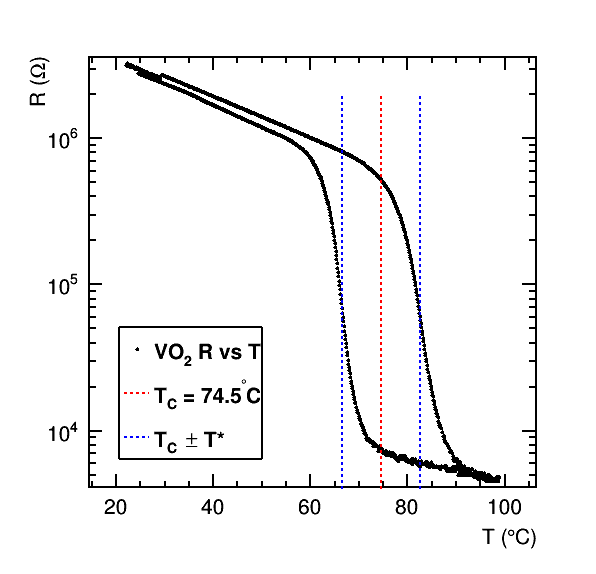
\includegraphics[width=0.4\textwidth]{VO2_RvT_withTC.png}
	\caption{Resistance vs Temperature Plot for $VO_{2}$ with Vertical Lines Identifying $T_{C}$ (Red) and $T_{C} \pm T^{*}$ (Blue)}
	\label{Fig:RvT1}
\end{figure}
\subsection{Ferroelectric Transition in $BaTiO_{3}$}

\section{Theoretical Model}

\section{Comparison of Theory and Experiment}

\section{Discussion and Conclusions}

\section{Author Contributions}

Both authors believe that the work for this project was split equally, and each offered valuable insight to every section of this report. However, the sections when divided up by principle author are as follows:

\noindent \textbf{Joshua LaBounty}:
\begin{enumerate}
	\item 
\end{enumerate}

\noindent \textbf{Thomas Krahulik}:
\begin{enumerate}
	\item Section 
\end{enumerate}

\noindent Lab time was also split equally, with one partner often taking measurements while the other developed the analysis software used in this report.

\begin{thebibliography}{6}
	
	\bibitem{milissinos}
	A.C. Melissinos, Experiments in Modern Physics (Academic Press, NY, 1966).
	
	\bibitem{bevington}
	Philip R. Bevington and D. Keith Robinson, Data Reduction and Error Analysis 3rd edition (McGraw-Hill, 2003).
	
	\bibitem{lab_manual}
	Mihaly, Laszlo and Gurvitch, Micheal. Phase Transitions: Metal-Insulator Transition in VO$_2$ and Ferroelectric Transition in BaTiO$_3$. (Stony Brook University, Nov. 14, 2014)

\end{thebibliography}

\begin{appendix}

\section{Validation of the $\chi^2$ Minimization in ROOT} \label{section:root}
For this experiment, we used ROOT, a c++ based data analysis software, to plot and fit functions to our data. To verify that ROOT calculates a correct value for $\chi^{2}$, we performed a hand calculation cross check with a simple set of data. The data set we used for this cross check was $\{ (11.0 \pm 0.0, 23.0 \pm 0.5), (14.0 \pm 0.0, 25.0 \pm 0.5), (20.0 \pm 0.0, 35.0 \pm 0.5), (25.0 \pm 0.0, 39.0 \pm 0.5) \}$. We plotted this data and fit it to a linear function $f(x) = [0] + [1]*x$. This plot is shown in Fig.~\ref{Fig:rootproof}.
\begin{figure}[H]
	\centering
	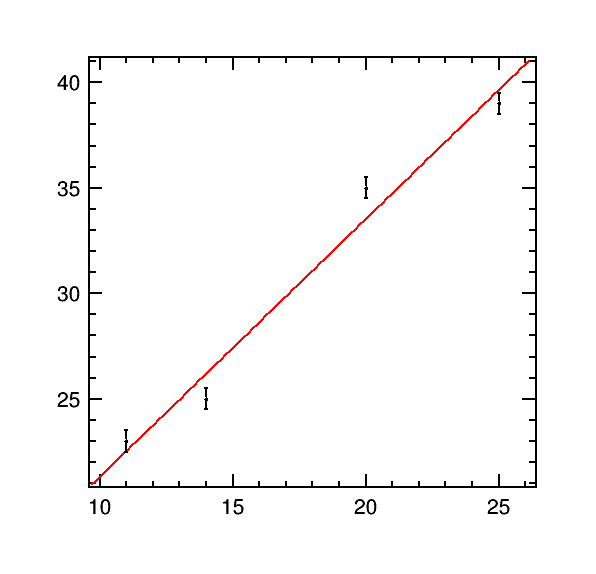
\includegraphics[width=0.4\textwidth]{rootproof.png}
	\caption{Sample Data Fitted to a Line}
	\label{Fig:rootproof}
\end{figure}
The function obtained from this fit was $f(x) = 9.11111 + 1.22222x$ with a chi-squared of $\chi ^{2} = 16.8889$. We then performed a hand calculation of the $\chi ^{2}$ using Eq.~\ref{eq:chisq}.
\begin{gather}\label{eq:chisq}
\chi ^{2} = \sum \frac{(f(x_i) - y_i)^{2}}{\sigma_i^2}
\end{gather}
When performing this hand calculation we also obtained a value of $\chi ^{2} = 16.8889$, verifying ROOT's ability to calculate $\chi ^{2}$.
\begin{align*}
\chi ^{2} =& \frac{(f(11.0) - 23.0)^{2}}{(0.5)^2} + \frac{(f(14.0) - 25.0)^{2}}{(0.5)^2} \\
&+ \frac{(f(20.0) - 35.0)^2}{(0.5)^2} + \frac{(f(25.0) - 39.0)^{2}}{(0.5)^2} \\
&= 16.8889
\end{align*}

\section{Analysis Code} \label{section:analysis_code}
All of the analysis code used for this lab can be found in the following git repository: 
\begin{verbatim}
https://github.com/jlabounty/SeniorLab/tree
/master/PhaseTransitions/
\end{verbatim}

\end{appendix}

\end{document}